\documentclass{article}
%\usepackage[latin1]{inputenc}
\usepackage{graphicx,amssymb,amsmath,amsbsy,MnSymbol} % extensions pour maths avancées
\usepackage{graphicx,mathenv}           % extensions pour figures
\usepackage[T1]{fontenc}        % pour les charactères accentués 
\usepackage[utf8]{inputenc} 
\usepackage{multicol}
\usepackage{wrapfig}
\usepackage{stmaryrd} % Pour les crochets d'ensemble d'entier
\usepackage{float}  % Pour placer les images là ou JE veux.

\DeclareMathOperator{\tr}{tr}
\DeclareMathOperator{\argmax}{argmax}
\DeclareMathOperator{\argmin}{argmin}
\DeclareMathOperator{\cov}{cov}


\setlength{\parindent}{0.0in}
\setlength{\parskip}{0.1in}
\setlength{\topmargin}{-0.4in}
\setlength{\topskip}{0.7in}    % between header and text
\setlength{\textheight}{9in} % height of main text
\setlength{\textwidth}{6in}    % width of text
\setlength{\oddsidemargin}{0in} % odd page left margin
\setlength{\evensidemargin}{0in} % even page left margin
%
%% Quelques raccourcis clavier :
\def\slantfrac#1#2{\kern.1em^{#1}\kern-.3em/\kern-.1em_{#2}}
\def\b#1{\mathbf{#1}}
\def\bs#1{\boldsymbol{#1}}
\def\m#1{\mathrm{#1}}
\bibliographystyle{acm}
%
\newcommand{\greeksym}[1]{{\usefont{U}{psy}{m}{n}#1}}
\newcommand{\inc}{\mbox{\small\greeksym{d}\hskip 0.05ex}}%
\pagenumbering{arabic}
\date{\today}
\title{Méthodes à noyaux - DM2}
\author{Nelle Varoquaux}
\begin{document}
\maketitle

\section{Exercice 1}
Soit $X = \(x_1, x_2, \dots, x_n\) \in \mathbb{R}^n$ et 
$Y = \(y_1, y_2, \dots, y_n\) \in \mathbb{R}^n$ . On définit:
\begin{equation*}
\cov_n (X, Y) = \mathbf{E}_n(XY) - \mathbf{E}_n(X)\mathbf{E}_n(Y)
\end{equation*}

avec $\mathbf{E}_n(U) = \(\sum_{i = 1}^n u_i / n\)$. Considérons par ailleurs
le critère suivant:

\begin{equation*}
C_n^K(X, Y ) = \max_{f, g \in \mathcal{B}_K} \cov_n(f(X), g(Y))
\end{equation*}

où $K$ est un noyau défini positif sur $\mathbb{R}$, $\mathcal{B_K}$ la
boule unité du RKHS de $K$, et $f(U) = (f(u_1), f(u_2), \dots, f(u_n))$

\subsection{Question 1}
Considérons le noyau linéaire : $K(a, b) = ab$.

\begin{align*}
C_n^K(X, Y ) & = & \max_{f, g \in \mathcal{B}_K} \cov_n(f(X), g(Y))
\end{align*}

On peut poser $f(x) = wx$ et $g(wx) = vx$. Or $f, g \in \mathcal{B}_K$. Donc
$\| w \| = \| v \|  = 1$, donc $w$ et $v$ valent $1$ ou $-1$.
On peut donc différencier 4 cas, $\cov_n(X, Y)$, $\cov_n(-X, Y)$, $\cov_n(X,
-Y)$, $\cov_n(X, -Y)$. On peut facilement en déduire que :

\begin{align*}
C_n^K(X, Y ) & = & |\cov_n(X, Y)) |
\end{align*}

\subsection{Question 2}

\section{Exercice 2}

Soit $(x_1, x_2, \dots, x_n) \in \mathbb{R}^p$. On veut créer $K$ cluster. On
pose $z^i$ les variables indiquant l'appartenance du point $i$ à un cluster.
La fonction coût est définie par:

\begin{equation*}
C_K(z, \mu) = \sum_{i = 1}^n \| x_i - \mu_{z_i}\|^2
\end{equation*}


\subsection{Question 1}

Afin de minimiser:

\begin{equation*}
\mu^k = \argmin_{\mu} C(z^i, \mu)
\end{equation*}

\begin{equation*}
z^{i + 1} = \argmin_z C(z, \mu^i)
\end{equation*}

On peut itérer avec les équations suivantes:
\begin{equation*}
z^i = \argmin_k \| x_i - \mu_k\|
\end{equation*}

\begin{equation*}
\mu^k = \frac{1}{N_k} \sum_{i \in C_k}x_i
\end{equation*}

\subsection{Question 2}
On veut maintenant trouver un algorithme itératif similaire sur le RKHS
$\mathcal{H}$, muni du noyau $K$ sur $\mathbb{R}^p$, i.e, minimiser:

\begin{equation*}
C_K(z, \mu) = \sum_{i = 1}^n \| \Phi(x_i) - \mu_{z_i}\|^2
\end{equation*}

où $\Phi : \mathbb{R^p} \rightarrow \mathcal{H}$ statisfait $\Phi(x)^T \Phi(x')
= K(x, x')$

On veut donc minimiser les deux équations suivantes:

\begin{equation*}
\mu^k = \argmin_{\mu} C(z^i, \mu)
\end{equation*}

\begin{equation*}
z^{i + 1} = \argmin_z C(z, \mu^i)
\end{equation*}

On peut donc itérer sur les deux équations suivantes:

\begin{align*}
z^i & = & \argmin_k \| x_i - \mu^k \|_{\mathcal{H}} \\
    & = & \argmin_k \( K(x_i, x_i) + K(\mu^k, \mu^k) - 2K(x_i, \mu^k)\)
\end{align*}

\begin{equation*}
\mu^k = \frac{1}{N_k} \sum_{i \in C_k} \Phi(x_i)
\end{equation*}

Donc :

\begin{align*}
z^i & = & \argmin_k \( K(x_i, x_i) + \frac{1}{N_k} \sum_{j \in C_k} K(x_j, x_j) - 2 \frac{1}{N_k}\sum_{j \in \mathcal{C}_k} K(x_i, x_j)\)
\end{align*}

\subsection{Question 3}

Soit $Z$ la matrice $n \times K$, comportant les valeurs $Z_{ij} = 1$ si $x_i$
est dans le cluster $j$ et 0 sinon. On pose par ailleurs $N_j = \sum_{i = 1}^n
Z_{ij}$ et $L$ la matrice diagonale $K \times K$, avec $L_{ii} =\frac{1}{N_i}$.
Montrons que minimizer $C_K(z, \mu)$ revient à maximiser:

\begin{equation*}
\tr \( L^{1/2}Z^T K Z L^{1/2} \)
\end{equation*}

On pose $M = \Phi Z L Z^T$, avec $\Phi$ matrice de taille $K \times n$, dont
les colonnes contiennent $\Phi(x_i)$. On peut donc en déduire que $\Phi^T \Phi
= K$
M est une matrice de taille $K$, contenant $\mu_k$. On
peut donc réécrire le coût tel que:

\begin{align*}
C_K & = & \tr \[ \(\Phi - M\)^T \( \Phi - M \) \] \\
    & = & \tr \[ \( \Phi - \Phi Z L Z^T \)^T \( \Phi - \Phi Z L Z^T\) \] \\
    & = & \tr \[ \Phi\(I - Z L Z^T \)^2 \Phi^T \]
\end{align*}

De plus, on a $Z^T Z = L^{-1}$, donc $(Z L Z^T)^2 = (Z L Z^T)$. De même 
$(I - ZLZ^T)^2 = (I - ZLZ^T)$. De plus, $L = L^{1/2} L^{1/2}$
Donc:

\begin{align*}
C_K & = & \tr \[ \Phi\(I - Z L Z^T \) \Phi^T \] \\
    & = & \tr \[ \Phi \Phi^T \] - \tr \[ \Phi Z L Z^T \Phi^T\] \\
    & = & \tr \[ K \] - \tr \[ \Phi Z L Z^T \Phi^T\] \\
    & = & \tr \[ K \] - \tr \[ K Z L Z^T \] \\
    & = & \tr \[ K \] - \tr \[ Z^T K Z L^{1/2} L^{1/2} \] \\
    & = & \tr \[ K \] - \tr \[ L^{1/2} Z^T K Z L^{1/2} \]
\end{align*}

Seul le deuxième terme de $C_K$ dépends de $Z$. Donc:

\begin{align*}
\min_Z C_K & = & \min_Z \{ \tr \[ K \] - \tr \[ L^{1/2} Z^T K Z L^{1/2} \] \} \\
	   & = & \min_Z \{ - \tr \[ L^{1/2} Z^T K Z L^{1/2} \] \} \\
	   & = & \max_Z \{ \tr \[ L^{1/2} Z^T K Z L^{1/2} \] \}
\end{align*}

\subsection{Question 4}

Posons $H = Z L^{1/2}$.

\begin{align*}
H^T H & = & \( Z L^{1/2} \)^T \( Z L^{1/2} \) \\
      & = & \( L^{1/2} \)^{T} Z^T Z L^{1/2}
\end{align*}

Or $L$ est diagonale, donc $\( L^{1/2} \)^{T} = L^{1/2}$. De plus, $Z^T Z = L^{-1}$. Donc:

\begin{align*}
H^T H & = & L^{1/2} L^{-1} L^{1/2} \\
      & = & I
\end{align*}

On peut donc reformuler le problème:

\begin{align*}
\max_Z \{ \tr \[ L^{1/2} Z^T K Z L^{1/2} \] \} & = & \max_Z \{ \tr \[ H^T K H \] \}
\end{align*}

avec $H H^T = I$.

On retrouve ici le problème du Kernel PCA, qui cherche à résoudre, $X$ étant
une matrice de donnée de taille $n \times d$

\begin{equation*}
var (h_w) = \frac{1}{n}\frac{w^T X^T X w}{w^T w}
\end{equation*}

Afin de maximiser $\max_Z \{ \tr \[ H^T K H \] \}$, on peut donc chercher les
$K$ plus grandes valeurs propres de $K$, et donc obtenir $C_K = \sum_{k = 1}^K
\lambda_k$.

On retrouve ici le problème du spectral clustering, qui consiste à extraire
des composantes principales grâce à l'algorithme ACP à noyau, et ensuite
appliquer un k-means sur les données projetées sur les composantes
principales.
% FIXME pas très clair tout ça, mais on retrouve le spectral clustering

\subsection{Question 5}

Implémentation de la question 2:
La première figure corresponds au cluster avec un K-means à noyau linéaire, la
deuxième figure, un kmeans à noyau gaussien.

\begin{figure}
\begin{center}
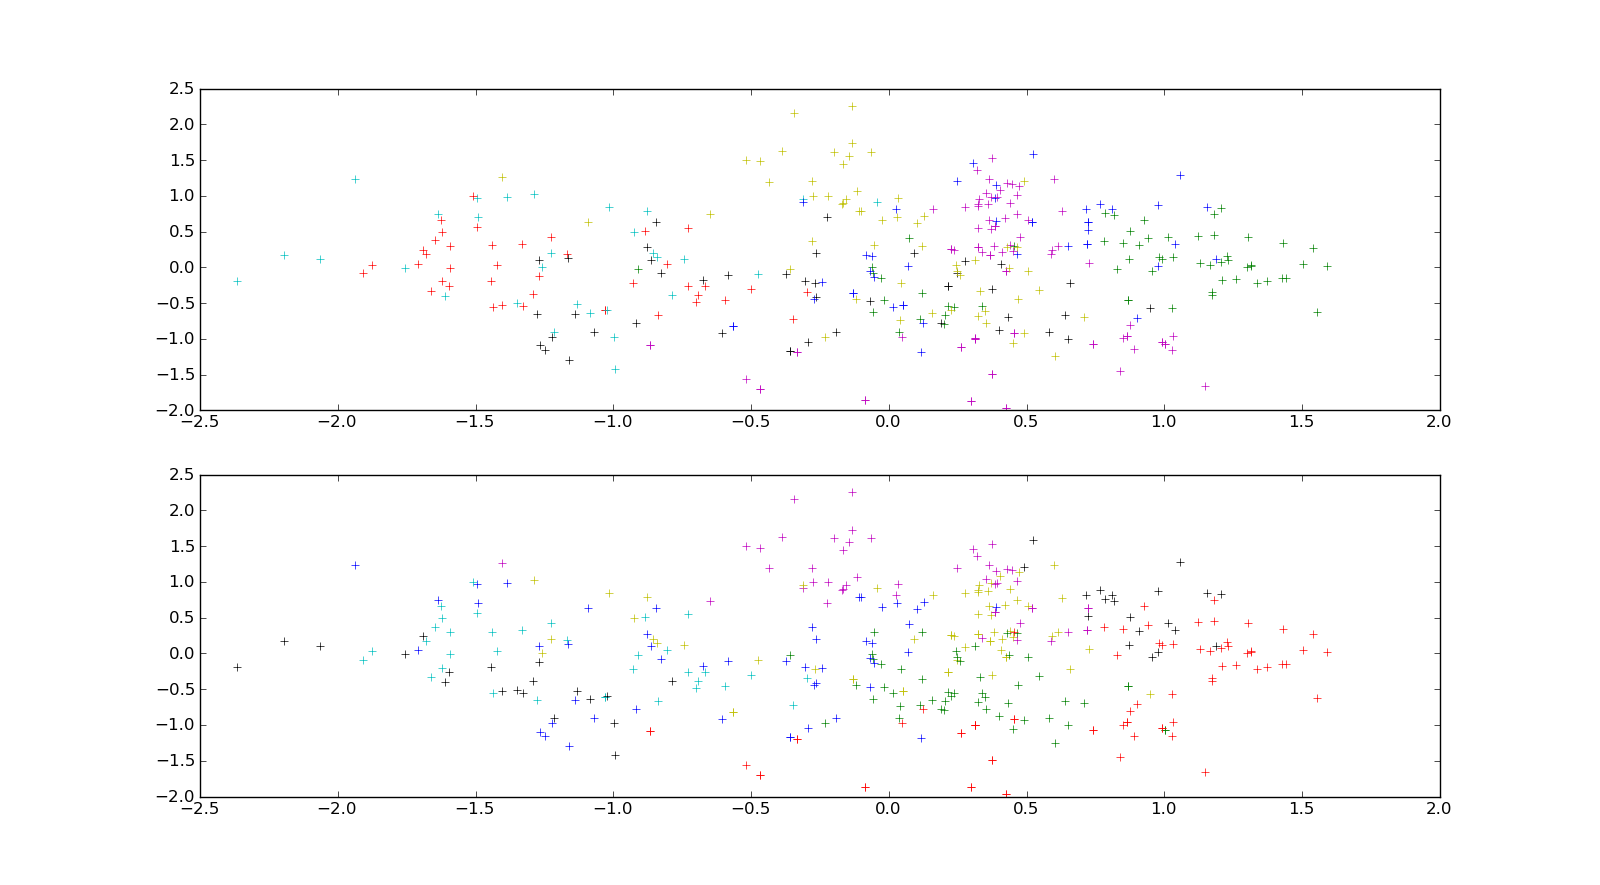
\includegraphics[width=550px]{./clusters.png}
\end{center}
\end{figure}

\end{document}
